
\documentclass[a4paper,11pt]{article}
\usepackage{float}
\usepackage{verbatim} 
\usepackage{graphicx}
\usepackage{hyperref }
\usepackage[acronym]{glossaries}
%\usepackage[xindy,toc]{glossaries}
\makeglossaries

\title{PyGMO Visualization Manual}
\author{
      Edgar Sim\'{o} Serra \\
      Mentored by Chit-Hong Yam and Dario Izzo 
}
\date{\today}

\begin{document}
\maketitle

\begin{abstract}
Manual for the Visualization module from PyGMO developed for PaGMO as part of the Google Summer of Code 2010 project.
\end{abstract}



\newacronym{API}{API}{Application Programmable Interface}
\newacronym{PaGMO}{PaGMO}{Parallel Global Multiobjective Optimizer}
\newglossaryentry{PyGMO}
{
   name={PyGMO},
   description={Python bindings for PaGMO}
}
\newacronym{GSoC}{GSoC}{Google Summer of Code}
\newglossaryentry{python}
{
   name={Python},
   description={Interpreted, object-oriented, high-level programming language with dynamic semantics}
}
\newglossaryentry{opengl}
{
   name={OpenGL},
   description={Standard specification defining a cross-language, cross-platform API for writing applications that produce 2D and 3D computer graphics}
}
\newacronym{CSV}{CSV}{Comma Separated Value}


% The glossary
\printglossaries


\tableofcontents
\newpage


\section{Introduction}
This is the manual for the Visualization module which is part of the \gls{PyGMO} python suite for interaction with \gls{PaGMO}\cite{pagmo}. The objective of this module is 3D Visualization of Interplanetary Trajectories. This manual is intended both for python developers using the PyGMO \gls{API} and end users executing the python script.


\subsection{Requirements}

The main requirement for the visualization module is \gls{python} and \gls{opengl}. Besides this the requirements are very loose. The following should give an approximate idea of what kind of computer is needed to run the visualization module:

\begin{itemize}
\item Pentium II class processor or better
\item 10 MB free dis space
\item 50 MB free RAM
\item OpenGL 1.1 capable card with VBO extension
\end{itemize}

To be able to run the visualization module you must have all the dependencies. The dependency list is:

\begin{itemize}
\item \gls{python}
\item PyOpengl module
\item numpy module
\item PyFTGL module
\item RE module
\item CSV module
\item dateutil module
\end{itemize}


\subsection{Features}

The Visualization module is designed around flexibility and simplicity. 

\paragraph{Feature list:}
\begin{itemize}
\item Visualization of trajectories
\item Ability to add planets
\item Time slider to be able to move to any time instant in the path
\item Keyboard interaction
\item Mouse Interaction that behaves like most 3D applications
\item Support for processing \gls{CSV} files.
\end{itemize}


\section{Installing the Visualization Module}

The installation is not different from the standard \gls{PaGMO} and \gls{PyGMO} installation\cite{install:pagmo}. However care must be taken so that \gls{PyGMO} is also installed.


\section{Using the Visualization Module}

The visualization module has two important aspects. The first is the acquiring of the data and setting up of the window. The second is the moving and manipulating of the trajectory with the window.


\subsection{Python API}

The \gls{python} \gls{API} is aimed at developers although it is simple enough to be used by anyone.

\subsubsection{Getting Started}

To get started with the python


\subsubsection{Advanced}


\subsubsection{Common Issues}


\subsection{3D Trajectory Window}


\subsubsection{Keybindings}


\subsubsection{Common Issues}


\section{Troubleshooting}


\appendix

\newpage
\section{example1.py}
Very simple example of an earth to mars trajectory.
\subsection{Data}
This example does not use external files for data, it declares the data in the code.
\subsection{Code}
\verbatiminput{../../example1.py}
\subsection{Results}
\begin{figure}[H]
\centering
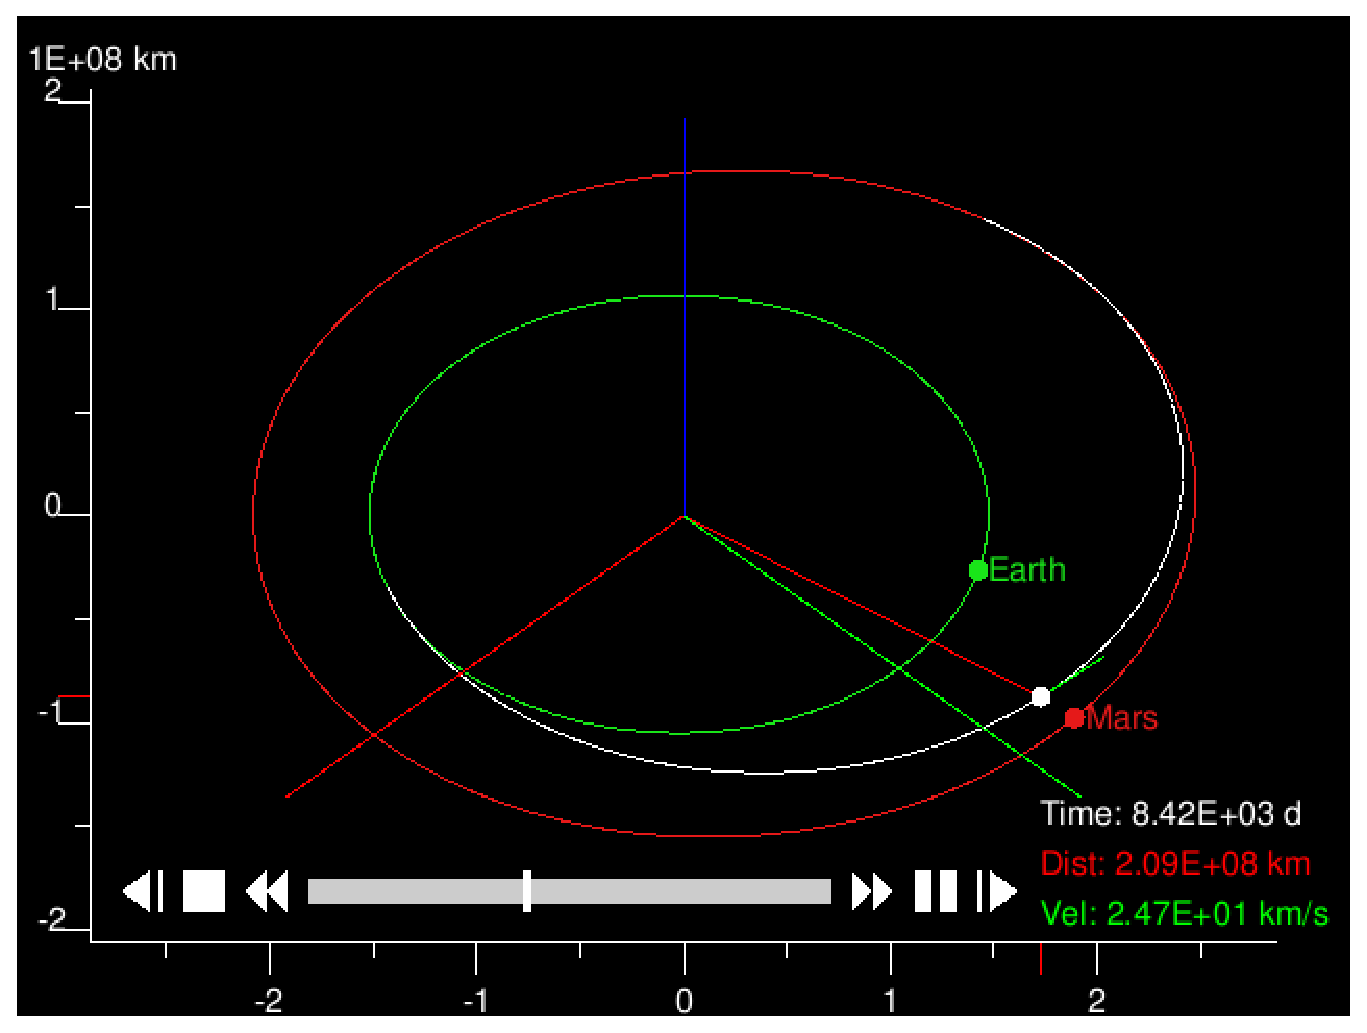
\includegraphics[width=1\textwidth]{img/example1}
\caption{Screenshot of the trajectory from example1.py}
\label{img:example1}
\end{figure}


\newpage
\section{example2.py}
Example of doing \gls{MGA}.
\subsection{Data}
For this example we are using:

\begin{itemize}
\item CassiniMGA.txt
\item CassiniMGA\_flybyinfo.txt
\end{itemize}
\subsection{Code}
\verbatiminput{../../example2.py}
\subsection{Results}
\begin{figure}[H]
\centering
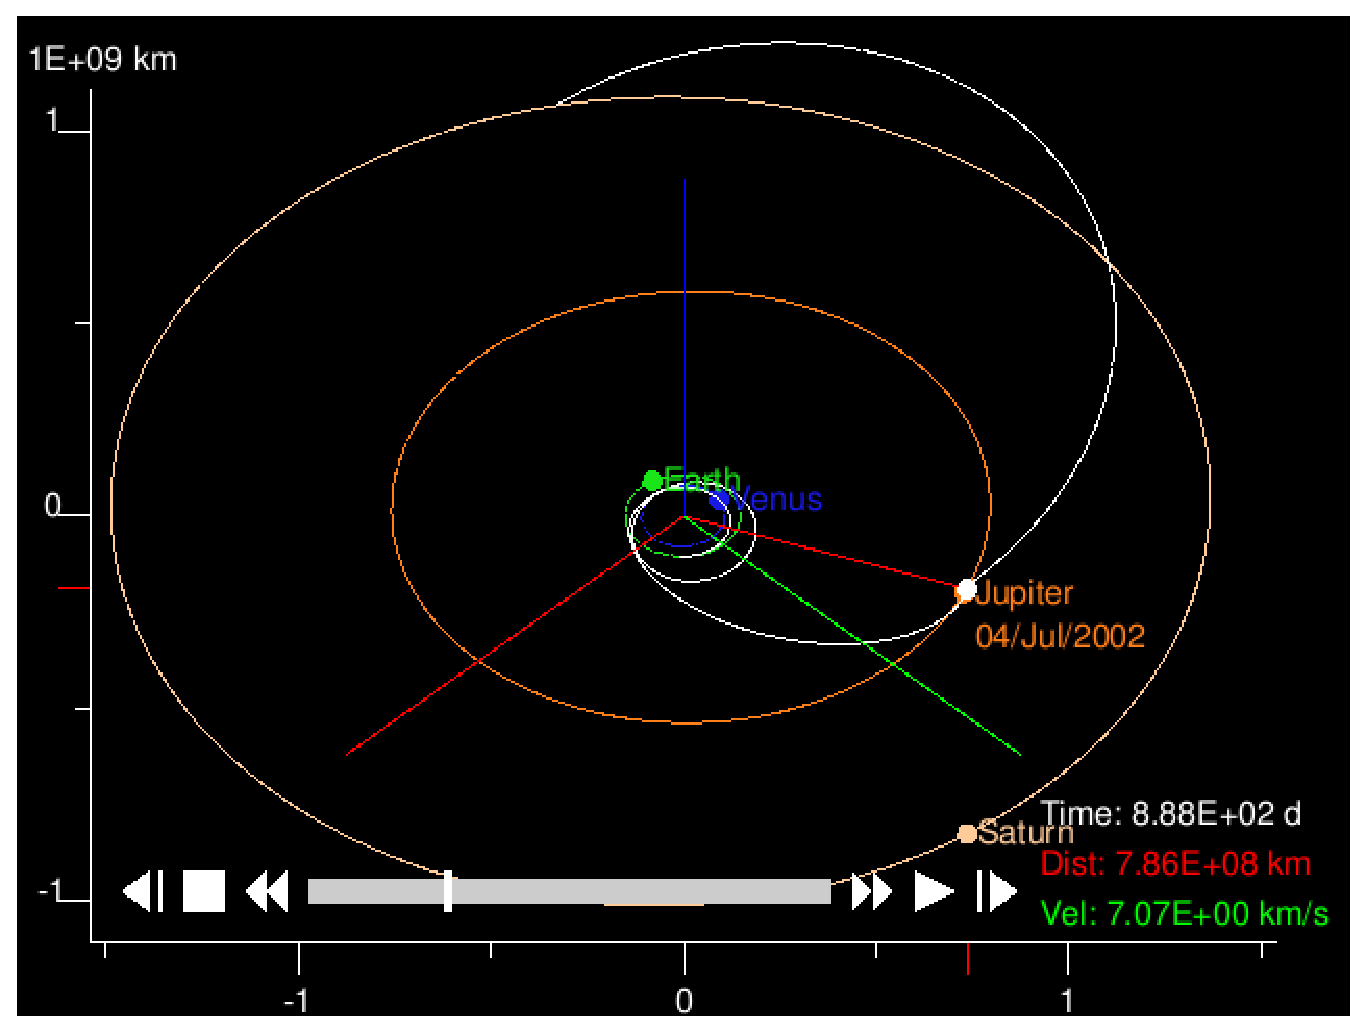
\includegraphics[width=1\textwidth]{img/example2}
\caption{Screenshot of the trajectory from example2.py}
\label{img:example2}
\end{figure}


\newpage
\section{example3.py}
Example of a simple \gls{DSM}.
\subsection{Data}
For this example we are using:

\begin{itemize}
\item EarthMarsDSM.txt
\item EarthMarsDSM\_flybyinfo.txt
\end{itemize}
\subsection{Code}
\verbatiminput{../../example3.py}
\subsection{Results}
\begin{figure}[H]
\centering
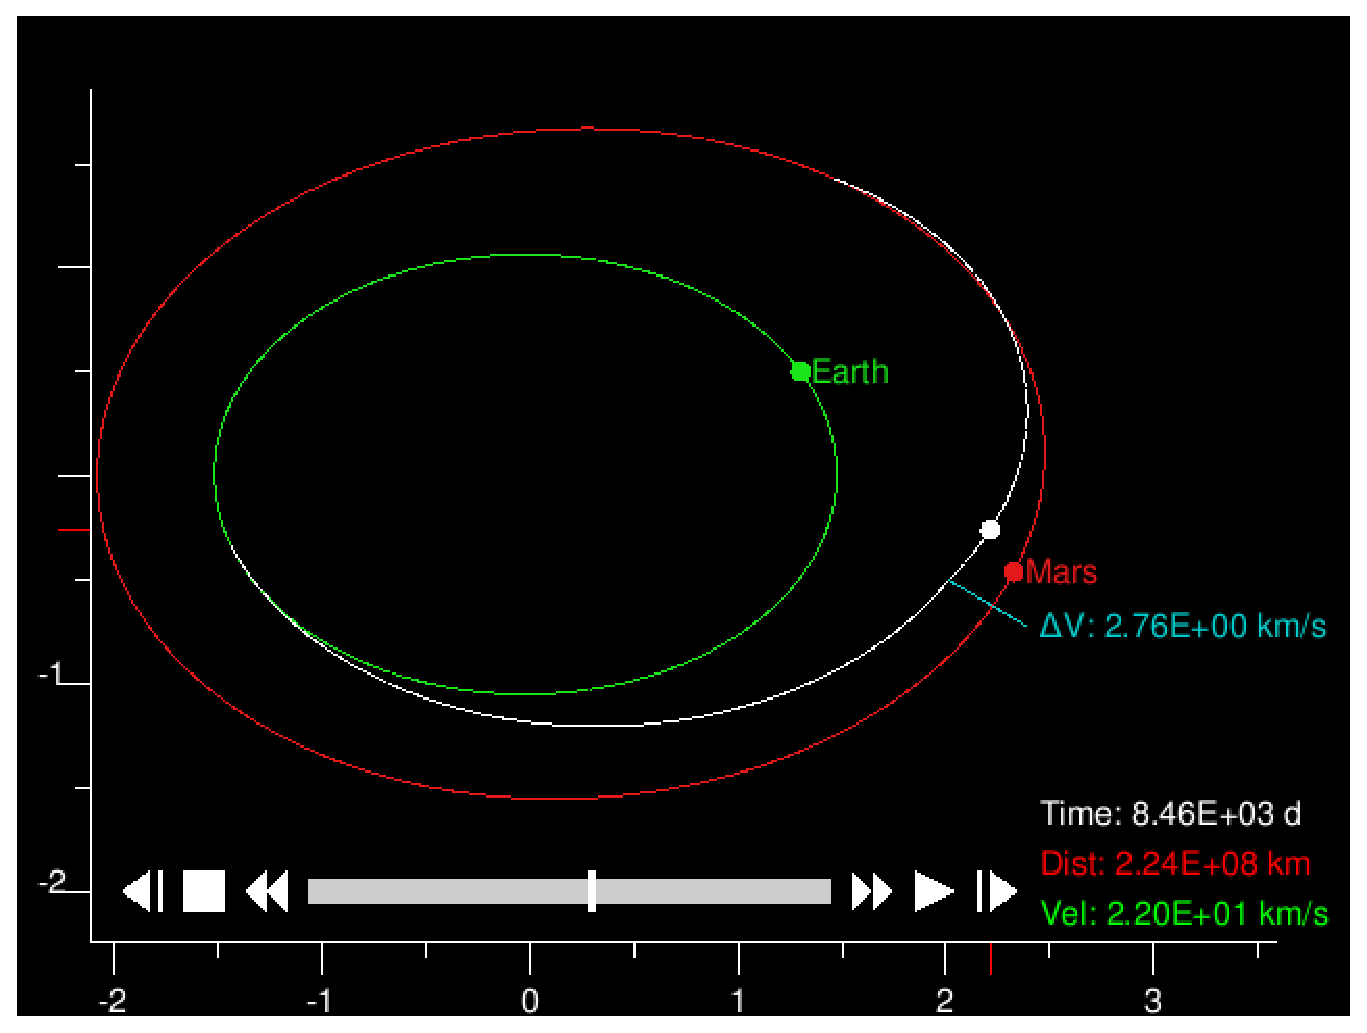
\includegraphics[width=1\textwidth]{img/example3}
\caption{Screenshot of the trajectory from example3.py}
\label{img:example3}
\end{figure}


\newpage
\section{example4.py}
Complete complex dataset example. This one does a gravity assist and multiple \gls{DSM}.
\subsection{Data}
For this example we are using:

\begin{itemize}
\item EarthEarthJupiter.csv
\item EarthEarthJupiter\_flybyinfo.txt
\end{itemize}
\subsection{Code}
\verbatiminput{../../example4.py}
\subsection{Results}
\begin{figure}[H]
\centering
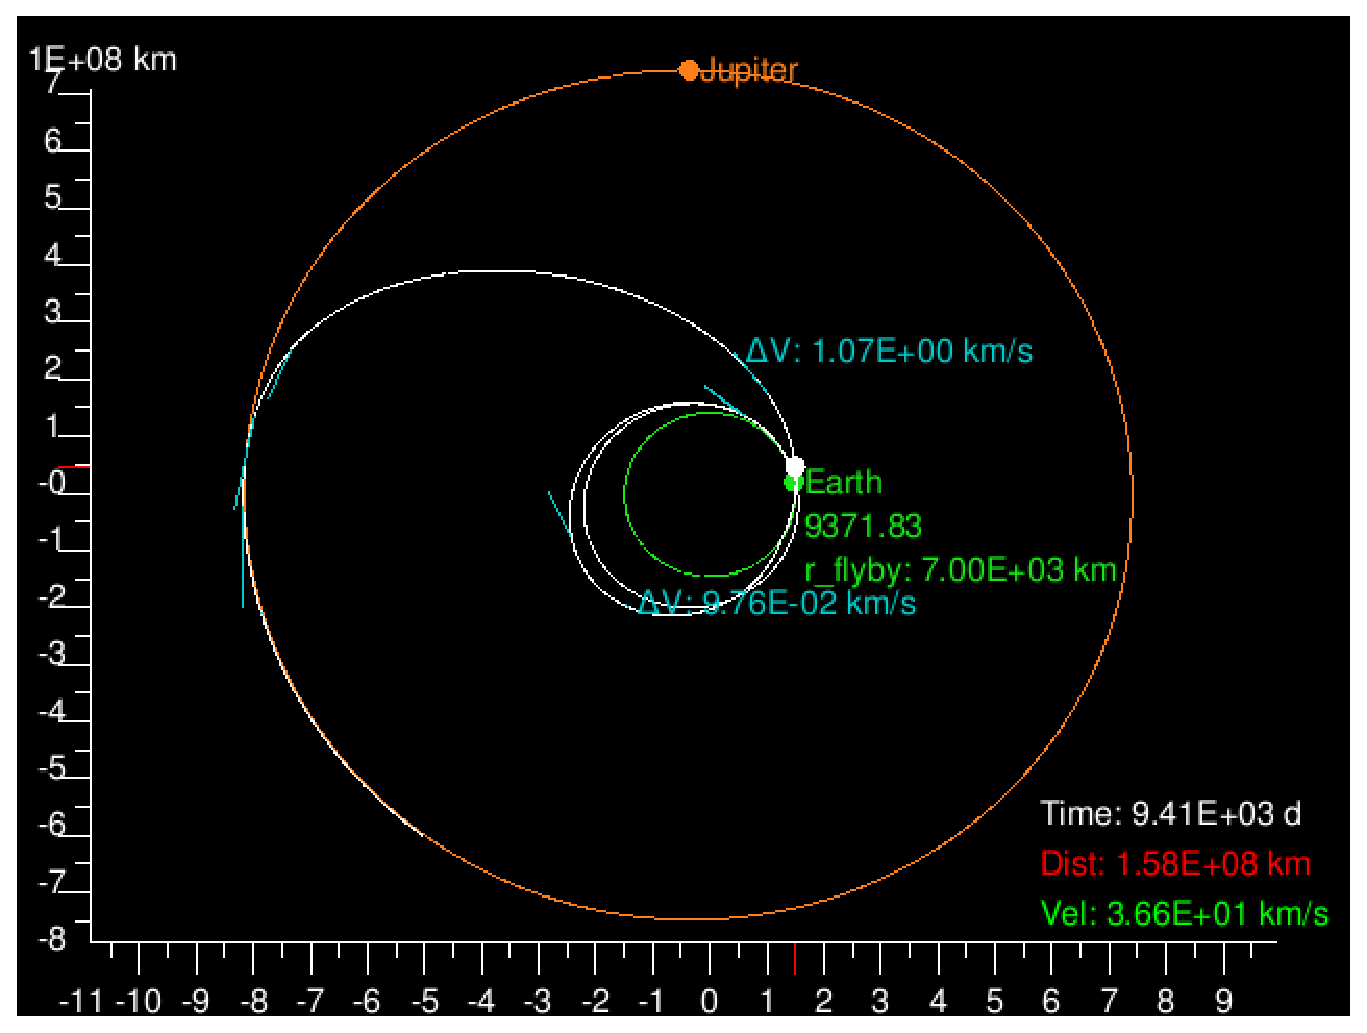
\includegraphics[width=1\textwidth]{img/example4}
\caption{Screenshot of the trajectory from example4.py}
\label{img:example4}
\end{figure}


\bibliographystyle{plain}
\bibliography{manbib}

\end{document}

